\documentclass[letterpaper,12pt,fleqn]{article}
\usepackage{matharticle}
\usepackage{pgfplots}
\pgfplotsset{compat=1.14}
\usepackage{siunitx}
\pagestyle{plain}
\begin{document}
\section*{Lab 7: The Difference Quotient}

The \emph{difference quotient} is an application of function algebra that is
very important to calculus students. It is given as follows:
\[\frac{f(x+h)-f(x)}{h}\]
Let's try an come up with some semantics for this bit of syntax. Consider the following
portion of the graph of some function:

\begin{minipage}{\textwidth}
  \centering
  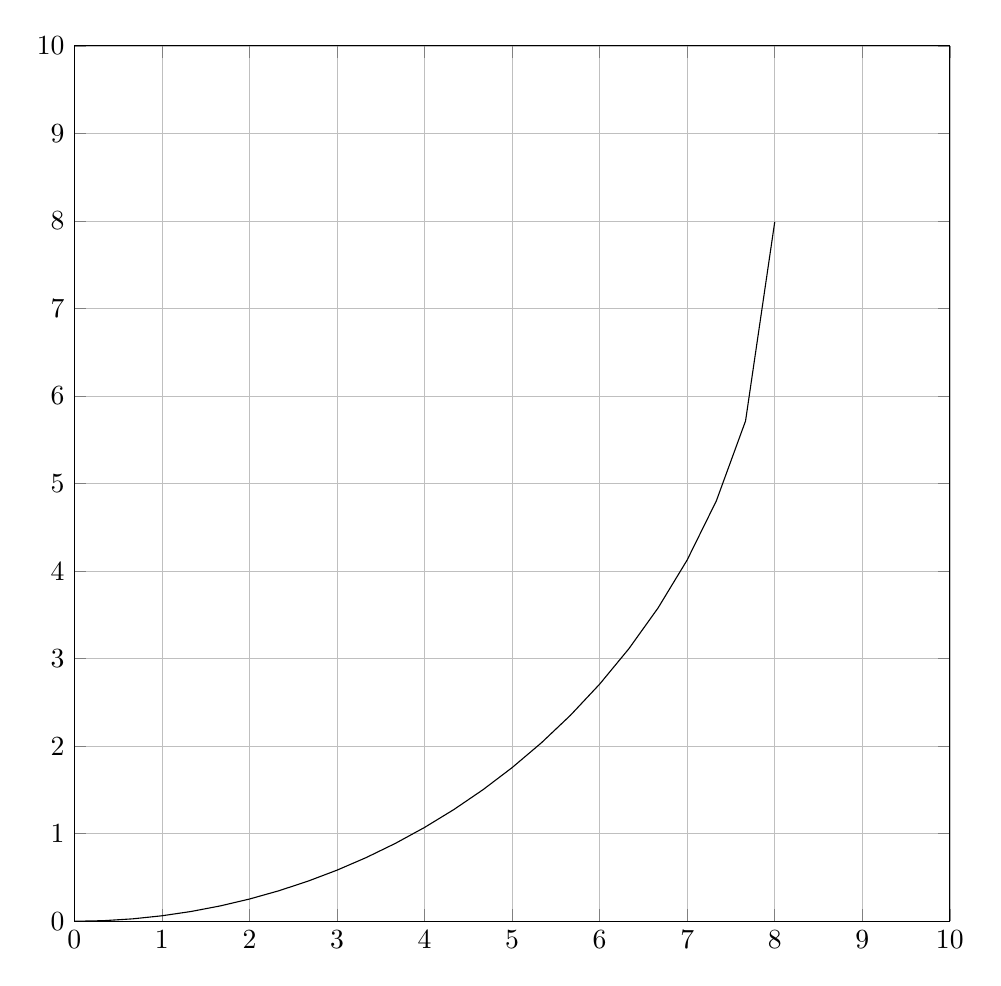
\begin{tikzpicture}
    \begin{axis}[
        width=5in,height=5in,
        xmin=0,xmax=10,
        ymin=0,ymax=10,
        grid=both,
        major grid style={line width=.2pt,draw=gray!50},
        axis line style={latex-latex},
      ]
      \addplot [domain=0:8] {-sqrt(64-x^2)+8};
    \end{axis}
  \end{tikzpicture}
\end{minipage}

Perform the following steps:
\begin{enumerate}
\item Plot the point $(5,f(5))$ on the graph.
\item Plot the point $(7,f(7))$ on the graph.
\item Draw the line that passes through the two plotted points.
\end{enumerate}

We call such a line through two points on a curve a \emph{chord}. Now look back at the
definition of the difference quotient and note that we can rewrite it as follows:
\[\frac{f(x+h)-f(x)}{h}=\frac{f(x+h)-f(x)}{(x+h)-x}\]
What you did was essentially draw a line through the points $(x,f(x))$ and $(x+h,f(x+h))$
where $x=5$ and $h=2$. Make sure that you see and understand this fact!

So what is the relationship between such a chord line on a graph and the difference
quotient? Examine the second form of the equation above and see if it reminds you of
anything that we did when we studied all about lines:

\vspace{1in}

Now image that we make $h$ smaller and smaller - i.e., arbitrarily small (there is that
phrase again!). What happens to the chord as $x+h$ gets closer and closer to $x$?

\vspace{1in}

The conclusion is that the difference quotient approaches the slope of the tangent line
as $h$ approaches $0$. This is the basis of differential calculus!

Here is an example. Consider the equation of a parabola:
\[y=x^2+3x-5\]
Let's calculate the difference quotient using function algebra:
\begin{eqnarray*}
  \frac{f(x+h)-f(x)}{h} &=& \frac{[(x+h)^2+3(x+h)-5]-(x^2+3x-5)}{h} \\
  &=& \frac{x^2+2xh+h^2+3x+3h-5-x^2-3x+5}{h} \\
  &=& \frac{2xh+3h+h^2}{h} \\
  &=& 2x+3+h
\end{eqnarray*}
Thus, when $h=0$, we get the slope of the tangent line at the point $x$:
\[m(x)=2x+3\]
Note how all the terms without an $h$ in them got canceled out. Thus, we were able to
divide all of the surviving terms by the $h$ in the denominator.

\newpage

Now you try. Find the slope of the tangent line at a point $x$ to the equation:
\[y=2x^2-x-3\]

\vspace{4in}

So big whoop. We can find the slope of the tangent line at a point in our curve. Here is
an example that shows why this is so important. What if our equation was an equation
of motion. Its graph would show how position changes with respect to time. Pick two
times: $t_0$ and $t_1$, which gives us two positions: $s(t_0)$ and $s(t_1)$. Let
$h=t_1-t_0$ and consider the equation:
\[\frac{s(t_0+h)-s(t_0)}{(t_0+h)-t_0}=\frac{s(t_0+h)-s(t_0)}{h}\]
But this is just out difference quotient! Furthermore, look at what we calculated: a
change in distance divided by a change in time --- this is velocity (speed)! Thus, the
difference quotient gives us the \emph{average} velocity between $t_0$ and $t_1$. But
this is just an average. The actual speed is changing constantly between those two times.
In fact, the slope of the tangent line at $t_0$ is called the \emph{instantaneous}
velocity at $t_0$.

Recall the equation of motion under gravity (in English units):
\[s=s_0+v_0t-16t^2\]
What is the velocity in ft/sec of a ball that is shot up from the ground with an
initial velocity of $\SI{100}{ft/s}$ after $2$ seconds?

Start by plugging in the given values for $s_0$ and $v_0$ into the equation of motion:
\[s=\]
Now, calculate the difference quotient:
\[\frac{s(t+h)-s(t)}{h}=\]

\vspace{4in}

Now let $h$ go to $0$:

\vspace{1in}

Now plug in $t=2$ to find the velocity of the ball after $2$ seconds:

\vspace{1in}

Congratulations! You have just done some calculus!
\end{document}
